\documentclass[25pt, a0paper, landscape, cmyk]{tikzposter}
% Fontspec changes the metrics slightly (!)
%\usepackage{fontspec}%\setsansfont{Montserrat Black}
% Use a simpler package instead
\input font-change-xetex
\mysanzfont{Montserrat Black}{30}{letterspace=6}
\usepackage[Export]{adjustbox}
\usepackage[colorlinks,allcolors=blue]{hyperref}
\tikzposterlatexaffectionproofoff
\title{One World, One Wiki}
\author{%
  C. Scott Ananian
  <cananian@wikimedia.org>
  \texttt{[[User:cscott]]}
  (Wikimedia Foundation)
}
\definecolorpalette{Wikimania2018}{
  % Red: 213 0 0 = D50000
  % Yellow: 255 193 7 = FFC107
  % Green: 0 174 66 = 00AE42
  \definecolor{colorOne}{HTML}{000000} % Black
  \definecolor{colorTwo}{HTML}{FFC107} % Yellow
  \definecolor{colorThree}{HTML}{D50000} % Red
  \definecolor{colorFour}{HTML}{00AE42} % Green
}
\definecolorstyle{CapeTown}{
  \definecolor{colorOne}{HTML}{FFC107}
  \definecolor{colorTwo}{HTML}{00AE42}
  \definecolor{colorThree}{HTML}{D50000}
}{  % Background Colors
    \colorlet{backgroundcolor}{colorOne}
    \colorlet{framecolor}{colorThree}
    % Title Colors
    \colorlet{titlefgcolor}{black}
    \colorlet{titlebgcolor}{white}
    % Block Colors
    \colorlet{blocktitlebgcolor}{colorTwo}
    \colorlet{blocktitlefgcolor}{black}
    \colorlet{blockbodybgcolor}{white}
    \colorlet{blockbodyfgcolor}{black}
    % Innerblock Colors
    \colorlet{innerblocktitlebgcolor}{colorFour}
    \colorlet{innerblocktitlefgcolor}{black}
    \colorlet{innerblockbodybgcolor}{white}
    \colorlet{innerblockbodyfgcolor}{black}
    % Note colors
    \colorlet{notefgcolor}{black}
    \colorlet{notebgcolor}{colorThree}
    \colorlet{notefrcolor}{colorThree}
}
\definecolorstyle{CapeTown2}{
  \definecolor{colorOne}{HTML}{FFC107}
  \definecolor{colorTwo}{HTML}{00AE42}
  \definecolor{colorThree}{HTML}{D50000}
}{  % Background Colors
    \colorlet{backgroundcolor}{colorTwo}
    \colorlet{framecolor}{colorThree}
    % Title Colors
    \colorlet{titlefgcolor}{black}
    \colorlet{titlebgcolor}{white}
    % Block Colors
    \colorlet{blocktitlebgcolor}{colorOne}
    \colorlet{blocktitlefgcolor}{colorTwo}
    \colorlet{blockbodybgcolor}{white}
    \colorlet{blockbodyfgcolor}{black}
    % Innerblock Colors
    \colorlet{innerblocktitlebgcolor}{colorFour}
    \colorlet{innerblocktitlefgcolor}{black}
    \colorlet{innerblockbodybgcolor}{white}
    \colorlet{innerblockbodyfgcolor}{black}
    % Note colors
    \colorlet{notefgcolor}{black}
    \colorlet{notebgcolor}{colorThree}
    \colorlet{notefrcolor}{colorThree}
}
\definecolorstyle{CapeTown3}{
  \definecolor{colorOne}{HTML}{FFC107}
  \definecolor{colorTwo}{HTML}{00AE42}
  \definecolor{colorThree}{HTML}{D50000}
}{  % Background Colors
    \colorlet{backgroundcolor}{colorFour}
    \colorlet{framecolor}{colorThree}
    % Title Colors
    \colorlet{titlefgcolor}{black}
    \colorlet{titlebgcolor}{white}
    % Block Colors
    \colorlet{blocktitlebgcolor}{colorOne}
    \colorlet{blocktitlefgcolor}{colorTwo}
    \colorlet{blockbodybgcolor}{white}
    \colorlet{blockbodyfgcolor}{black}
    % Innerblock Colors
    \colorlet{innerblocktitlebgcolor}{colorTwo}
    \colorlet{innerblocktitlefgcolor}{black}
    \colorlet{innerblockbodybgcolor}{white}
    \colorlet{innerblockbodyfgcolor}{black}
    % Note colors
    \colorlet{notefgcolor}{black}
    \colorlet{notebgcolor}{colorThree}
    \colorlet{notefrcolor}{colorThree}
}


\usetheme{Default}
\usecolorstyle[colorPalette=Wikimania2018]{CapeTown2}
\useinnerblockstyle{Table}

% remove space taken up by \institute
\settitle{ \centering \vbox{
\centering
\color{titlefgcolor} {\sanstwentycaps \@title \par}
\vspace*{1em}
{\huge \@author}
}}
\newcommand{\myb}[1]{\sanssixteencaps #1}

% Work around tikzposter conflict with hyperref
% https://tex.stackexchange.com/questions/254257/tikzposter-and-doi-package-conflict
\def\HyperFirstAtBeginDocument#1{#1}
\begin{document}\maketitle[width=90cm,titletotopverticalspace=0.5cm,titletoblockverticalspace=1cm]
\block{}{\centering
  Instead of today's many siloed wikis, separated by language and
  project, we aspire to re-establish a unified community of
  collaborators in the spirit of \textit{ubuntu}. We will still respect
  language and cultural differences---there will still be English,
  German, Hebrew, Arabic, etc. Wikipedias; they will disagree at
  times---but
  instead of separate domains, we propose a single user
  experience with integrated navigation between projects and languages
  and the possibility of split screen views aligning related
  content. On a single page we can work on articles in different
  languages, or simultaneously edit textbook content and encyclopedia
  articles. Via machine translation we can facilitate conversations
  and collaborations spanning languages and projects, without forcing
  a single culture or perspective.
  %The improvements made to the
  %project by each community can be shared with all others to improve
  %the sum of all knowledge.
  }
\begin{columns}
  \column{0.5}
  \newlength{\myfigwidth}
  \setlength{\myfigwidth}{0.34\colwidth}
  \newlength{\myfiggap}
  \setlength{\myfiggap}{1.5cm}
  \block{\myb{Language Converter}}{

    MediaWiki uses
    \href{https://www.mediawiki.org/wiki/Writing_systems\#LanguageConverter}{[[mw:LanguageConverter]]}
    to automatically transliterate articles between closely related
    languages/dialects or script variants of a language/dialect.
    It is used on 11 wikis, and has been requested on about 35 more.
    Some examples of conversion pairs:

    \innerblock{%
      \raisebox{0pt}[0pt][0pt]{\parbox{13cm}{\raggedright%
          English (American/British)\\\rm
          \textit{LanguageConverter not used.}

          Spelling and usage differences exist between American
          English, British English, Indian English, and others.
      }}%
    }{%
      \includegraphics[valign=T,width=\myfigwidth]{variants-en-us.eps}%
      \hspace{\myfiggap}%
      \includegraphics[valign=T,width=\myfigwidth]{variants-en-gb.eps}%

      \vspace{1cm}
    }
    \innerblock{
      \raisebox{0pt}[0pt][0pt]{\parbox{13cm}{\raggedright%
          Serbian (Latin/Cyrillic)\\\rm
          \textit{LanguageConverter in use.}

          Speakers are fully functionally digraphic, using both
          Cyrillic and Latin scripts.  There are vocabulary
          differences between Ikavian, Ekavian, and Ijekavian dialects
          which are not currently converted.
      }}%
    }{%
      \includegraphics[valign=T,width=\myfigwidth]{variants-sr-el.eps}%
      \hspace{\myfiggap}%
      \includegraphics[valign=T,width=\myfigwidth]{variants-sr-ec.eps}%
    }
    \innerblock{
      \raisebox{0pt}[0pt][0pt]{\parbox{13cm}{\raggedright%
          Chinese (Simplified/Traditional)\\\rm
          \textit{LanguageConverter in use.}

          Simplified used in mainland China, Singapore, and
          Malaysia.  Traditional used in Taiwan, Hong Kong,
          Macau, and among Overseas Chinese.
          Most speakers monographic; few can fluently
          proofread text in both variants.
        }}%
    }{%
      \includegraphics[valign=T,width=\myfigwidth]{variants-zh-cn.eps}%
      \hspace{\myfiggap}%
      \includegraphics[valign=T,width=\myfigwidth]{variants-zh-tw.eps}%

      \vspace{7cm}
    }
    \innerblock{
      \raisebox{0pt}[0pt][0pt]{\parbox{13cm}{\raggedright%
          Hindi/Urdu\\\rm
          \textit{LanguageConverter not used.}

          Urdu and Hindi are dialects of the Hindustani language,
          written in very different scripts: Arabic on the Pakistan
          side of the border, Devanagri on the India side.
%          (Punjabi is a similar case, with four scripts used.)

          Currently separate small wikis; could combine efforts.
        }}%
    }{%
      \includegraphics[valign=T,width=\myfigwidth]{variants-hi.eps}%
      \hspace{\myfiggap}%
      \includegraphics[valign=T,width=\myfigwidth]{variants-ur.eps}%

      \vspace{0.5cm}
    }

    %\small LanguageConverter brings our wikis together!
  }
  \column{0.5}
  \block{\myb{Native Variant Editing}}{

    LanguageConverter is oriented to readers: it converts the article
    text unidirectionally into readable text in a consistent variant.
    But as soon as a user begins to edit, they are confronted with the
    source text in a mix of variants, as illustrated by the
    intermingled Cyrillic and Latin scripts in the article from
    Serbian Wikipedia shown below.  This mixture of scripts can be a
    huge barrier to editing in communities where individuals are
    typically only fluent in a single variant.

    \quad The Parsoid team has been experimenting with a new bidirectional
    implementation of LanguageConverter, based on Finite State
    Transducers (FSTs).  These allow automatic annotation of wikitext
    such that it can be round-tripped to its original variant
    losslessly.  With these annotations, an Wikimedian can edit an
    article in their preferred consistent variant.
    Unedited portions of the article will round-trip to their original
    variant, preventing dirty diffs.

    \quad On wikis where the
    community has chosen to author all articles in a single variant,
    all text can be losslessly saved as the chosen variant, regardless
    of which variant the editor used.

    \begin{center}
    \textbf{We can make editing easier on wikis using LanguageConverter!}
    \end{center}

    \begin{tikzfigure}
      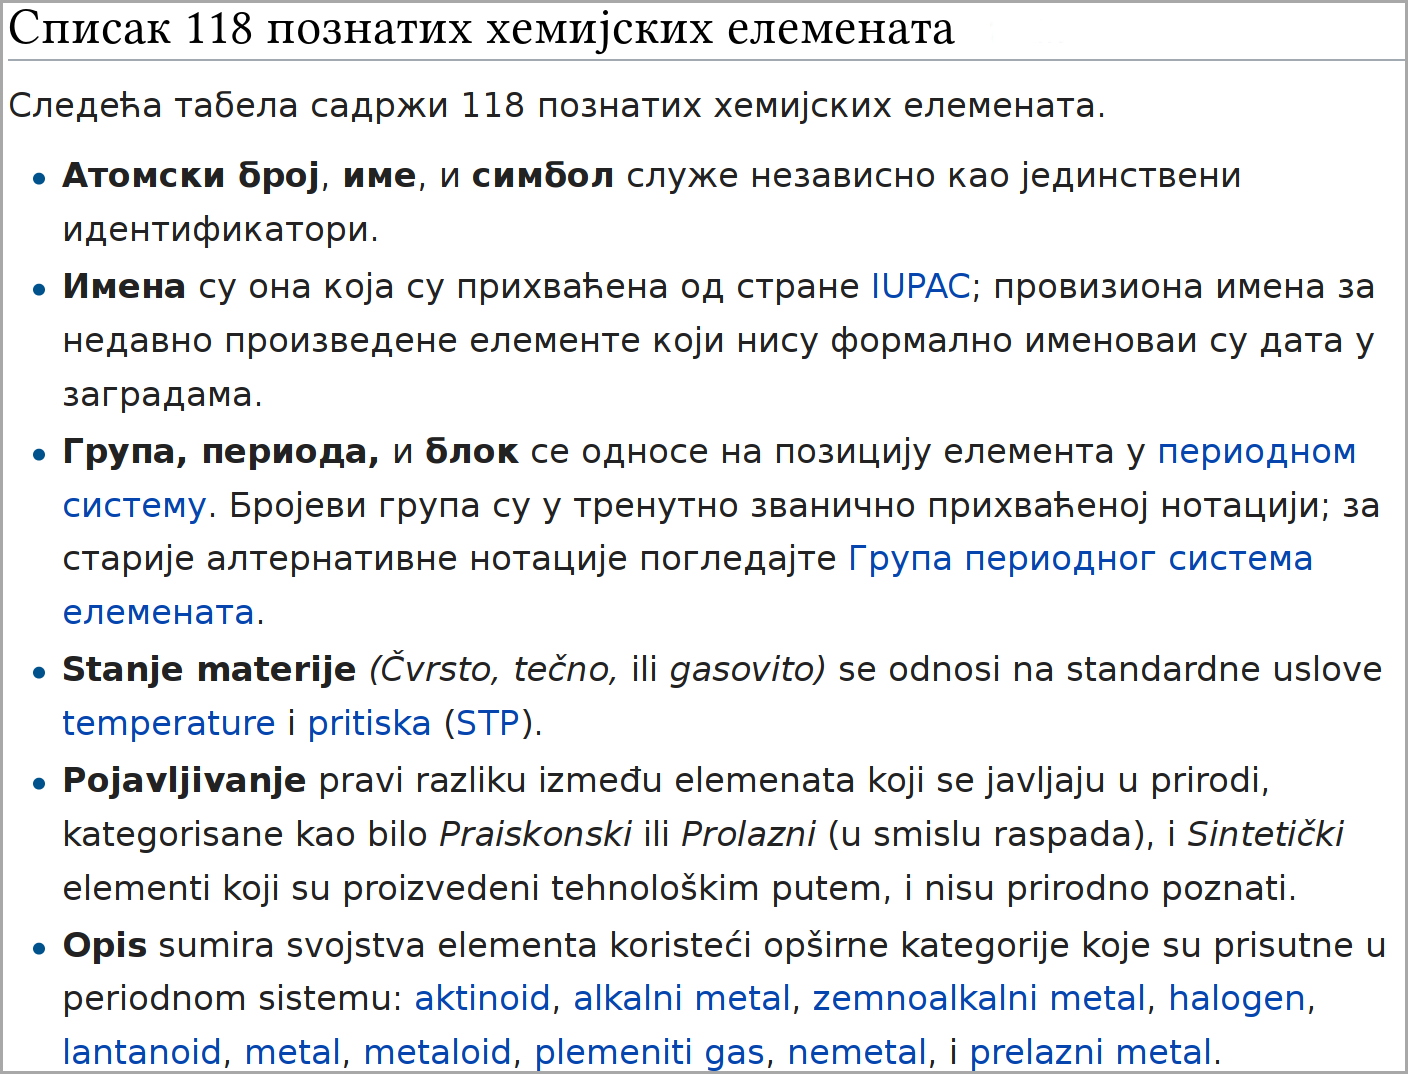
\includegraphics[height=17.25cm,valign=T]{mixed-edit-2.png}
      \hspace{7.5cm}
      \includegraphics[height=17.25cm,valign=T]{simple.eps}

      \vspace{0.75cm}

      \parbox[t]{26cm}{Serbian Wikipedia article showing mixed
        Cyrillic/Latin script}
      \hspace{2cm}
      \parbox[t]{22cm}{Partial FST for Serbian Cyrillic-to-Latin
        conversion}
    \end{tikzfigure}
  }
  \block{\myb{Translation Suggestion Tool}}{

    A translation suggestion tool \textbf{suggests an edit in one
      language whenever an edit is made to a parallel text in another
      language}.  Correspondences are
    \href{https://www.mediawiki.org/wiki/Content_translation/Published_translations\#Parallel_corpora}{manually created}
    via the Content Translation tool or
    \href{http://www.statmt.org/wmt17/bandit-learning-task.html}{``bandit learning''},
    and machine translation is used to automatically
    create new (or prune old) correspondences.

    \centering
    Related work: \url{https://research.wikimedia.org/knowledge-gaps.html}
  }
  \block{\myb{Zero-Shot Translation}}{

    ``Zero-shot translation'' machine translation models \textbf{allow
      training data from ``big'' wikis to improve the translation of
      ``small'' wikis}. Every contributed correspondence or
    translation further improves the ability of our tools to make
    additional articles from other languages available.

    \centering
    More information: \url{https://arxiv.org/pdf/1611.04558.pdf}

  }
  \block{}{\centering\bf
    By bridging languages, our individual contributions can better fill
    knowledge gaps everywhere.
  }
\end{columns}
\end{document}
